\documentclass{article}
\usepackage[utf8]{inputenc}
\usepackage[margin=1in]{geometry}
\usepackage[portuguese]{babel}
\usepackage{graphicx}
\usepackage{amsmath}
\graphicspath{ {./images/} }

\title{Sinais e Sistemas - Trabalho 1 - Grupo 2}
\author{
    Leonardo Soares da Costa Tanaka \\
    Matheus Henrique Sant Anna Cardoso \\
    Theo Rudra Macedo e Silva
}

\date{Setembro de 2022}

\begin{document}

\maketitle

1.) Para o sinal abaixo, contínuo por partes e definido para $t \in [-5\;5]$: (a) esboçar gráfico, (b) encotrar uma expressão analítica usando sinais singulares, (c) escrever um programa que rode em Octave/MatLab para plotar o gráfico. Nos dados a seguir, as expressões entre vírgulas se referem, na ordem de apresentação, aos valores do sinal nos intervalos $I_{1} = [-5\;-3], I_{2} = [-3\;-1], I_{3} = [-1\;1], I_{4} = [1\;3], I_{5} = [3\;5]$.
\textbf{G2}: $x(t) = -3, 3t + 6, -3t^3, 3t - 6, -t^2 + 5t - 3$

\vspace{\baselineskip}

(a) Esboçando o gráfico:

\begin{figure}[h]
    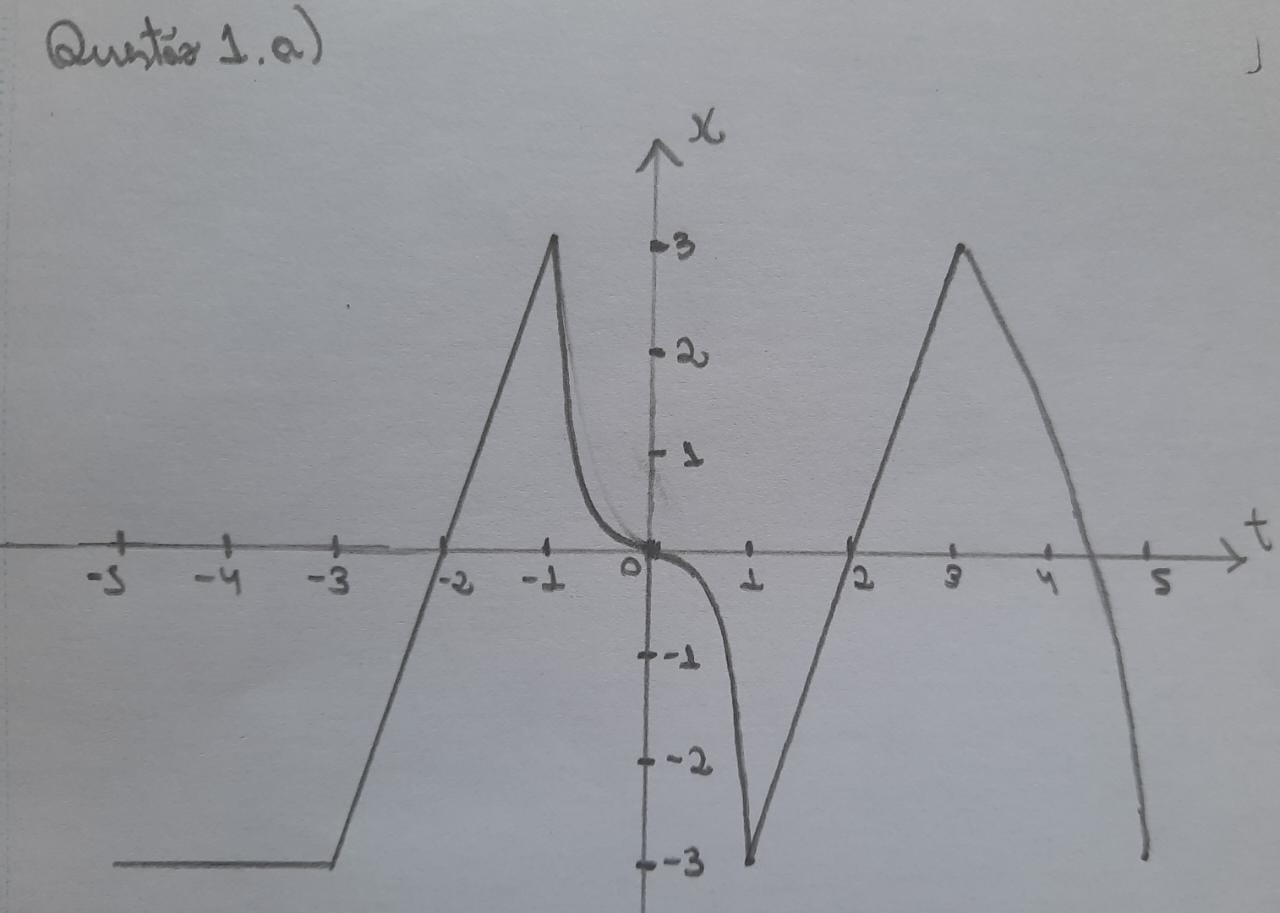
\includegraphics[scale=0.23]{plot1a}
    \centering
\end{figure}

\vspace{\baselineskip}

(b) Analisando para os intervalos, teremos:

\vspace{\baselineskip}

Para $ -5 \leq t < -3, x(t) = -3 $, ou, $ x(t) = -3 \cdot 1(-t) $ utilizando um degrau refletido.

\vspace{\baselineskip}

Para $ -3 \leq t < -1, x(t) = 3t + 6 $, ou, $ x(t) = 3t \cdot 1(-t) + 6 \cdot 1(-t) $ utilizando degrau e rampa unitários.

\vspace{\baselineskip}

Para $ -1 \leq t < 0, x(t) = -3t^3 $, ou, $ x(t) = -6t \cdot \frac{t^2}{2}1(-t) $ utilizando a parábola unitária.

\vspace{\baselineskip}

Para $ 0 \leq t < 1, x(t) = -3t^3 $, ou, $ x(t) = -6t \cdot \frac{t^2}{2}1(t) $ utilizando a parábola unitária.

\vspace{\baselineskip}

Para $ 1 \leq t < 3, x(t) = 3t - 6 $, ou, $ x(t) = 3t \cdot 1(t) - 6 \cdot 1(t) $ utilizando degrau e rampa unitários.

\vspace{\baselineskip}

Para $ 3 \leq t < 5, x(t) = -t^2 + 5t - 3 $, ou, $ x(t) = -2 \cdot \frac{t^2}{2}1(t) + 5t \cdot 1(t) - 3 \cdot 1(t)$ utilizando parábola, rampa e degrau unitários.

\vspace{\baselineskip}

Dessa forma, teremos $x(t)$ definido como:

\[ x(t) = 
\begin{cases} 
    -3 \cdot 1(-t) & -5 \leq t < -3 \\

    3t \cdot 1(-t) + 6 \cdot 1(-t) & -3 \leq t < -1 \\

    -6t \cdot \frac{t^2}{2}1(-t) & -1 \leq t < 0 \\

    -6t \cdot \frac{t^2}{2}1(t) & 0 \leq t < 1 \\

    3t \cdot 1(t) - 6 \cdot 1(t) & 1 \leq t < 3 \\

    -2 \cdot \frac{t^2}{2}1(t) + 5t \cdot 1(t) - 3 \cdot 1(t) & 3 \leq t < 5 
 \end{cases}
\]


\vspace{\baselineskip}

(c) Executando os códigos escritos no Octave, plotamos o seguite gráfico:

\begin{figure}[h]
    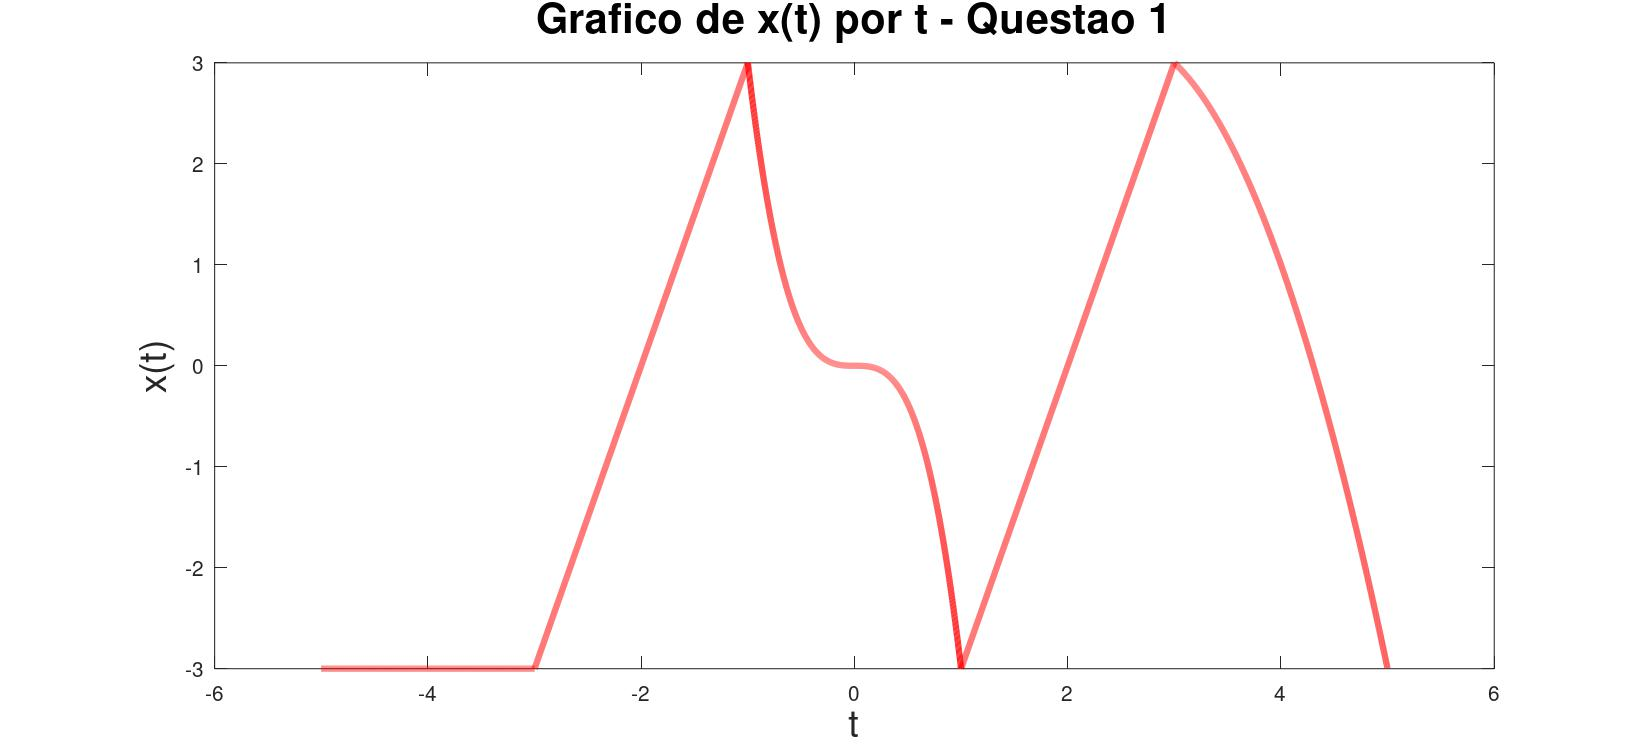
\includegraphics[scale=0.23]{plot1c}
    \centering
\end{figure}

2.) Plotar o gráfico dos sinais a seguir, com escalas adequadas e usando os valores numéricos desejados para os eventuais parâmetros. Dizer se estes sinais são periódicos e, em caso afirmativo quais os seus períodos fundamentais.
(a) $x(t) = sen(\pi t) + cos(2 \pi t) / 2 + sen(3 \pi t) / 3 + cos(4 \pi t) / 4$,
(b) $x(t) = sen(\omega t)cos(50\omega t)$,
(c) $x(t) = sen(\omega t^2)$,
(d) $x(t) = sen(\omega_{1}sen(\omega_{2}t)t)$

\vspace{\baselineskip}

(a) Plotando o gráfico no Octave, temos:

\vspace{\baselineskip}

\begin{figure}[h!]
    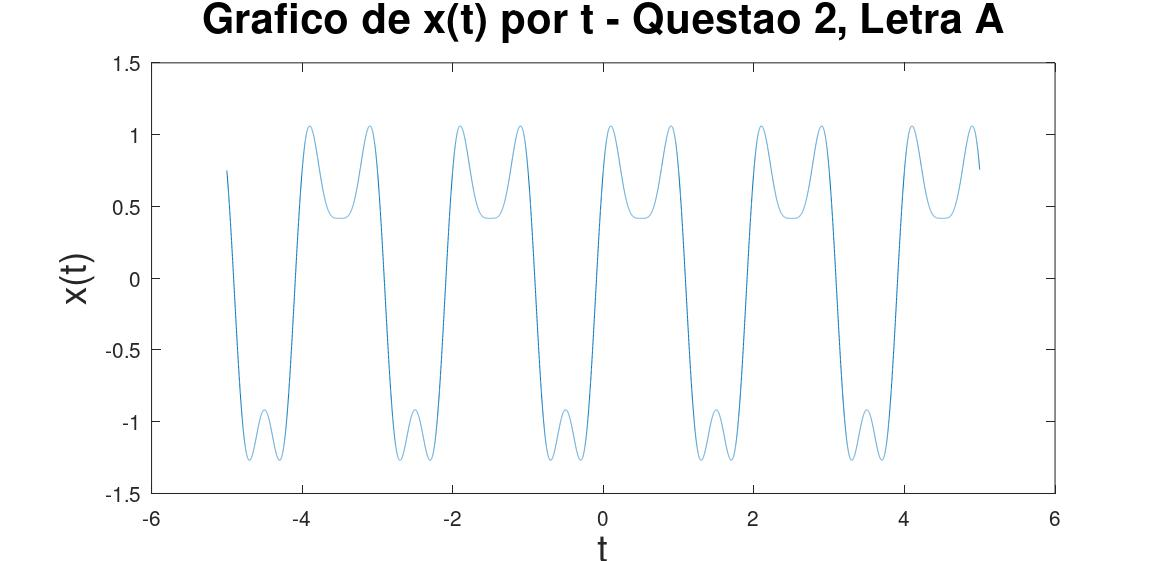
\includegraphics[scale=0.3]{plot2a}
    \centering
\end{figure}

\newpage

(b) Plotando o gráfico no Octave, temos:

\vspace{\baselineskip}

\begin{figure}[h!]
    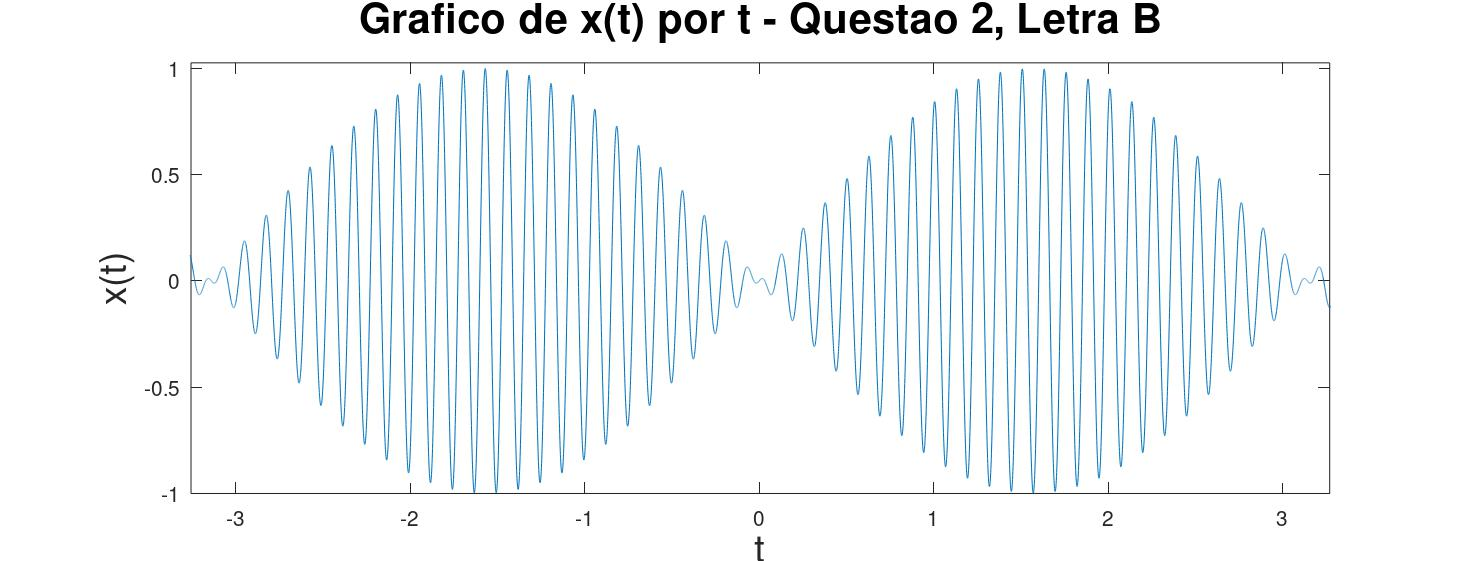
\includegraphics[scale=0.25]{plot2b}
    \centering
\end{figure}

\vspace{\baselineskip}

(c) Plotando o gráfico com o Octave para $\omega = 7$, temos:
\begin{figure}[h!]
    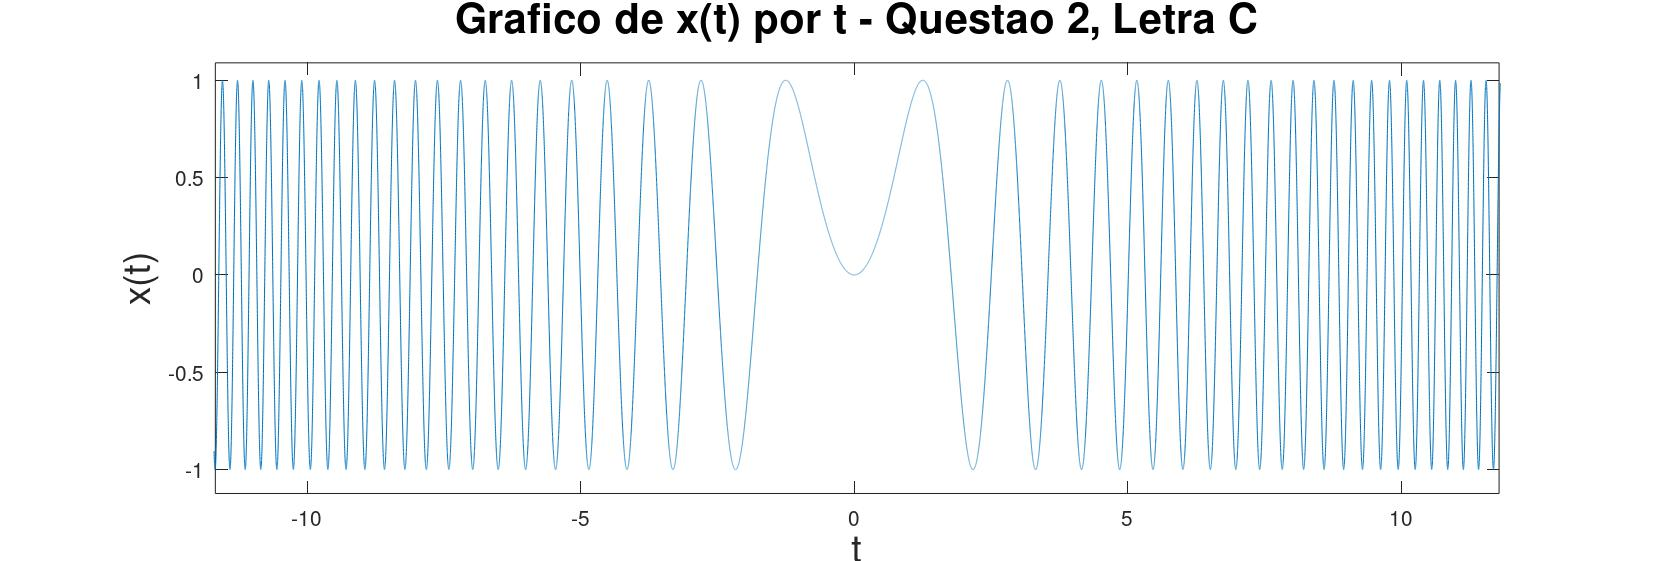
\includegraphics[scale=0.2]{plot2c}
    \centering
\end{figure}

Daqui, já se nota que o sinal não é periódico. Além de ser bem destoante para valores próximos à zero, conforme $t \rightarrow \infty$ ou $t \rightarrow - \infty$, a distância entre as cristas e entre os vales diminui.

\vspace{\baselineskip}

(d) Plotando o gráfico com o Octave para $\omega_{1} = \omega_{2} = 1$, temos:
\begin{figure}[h!]
    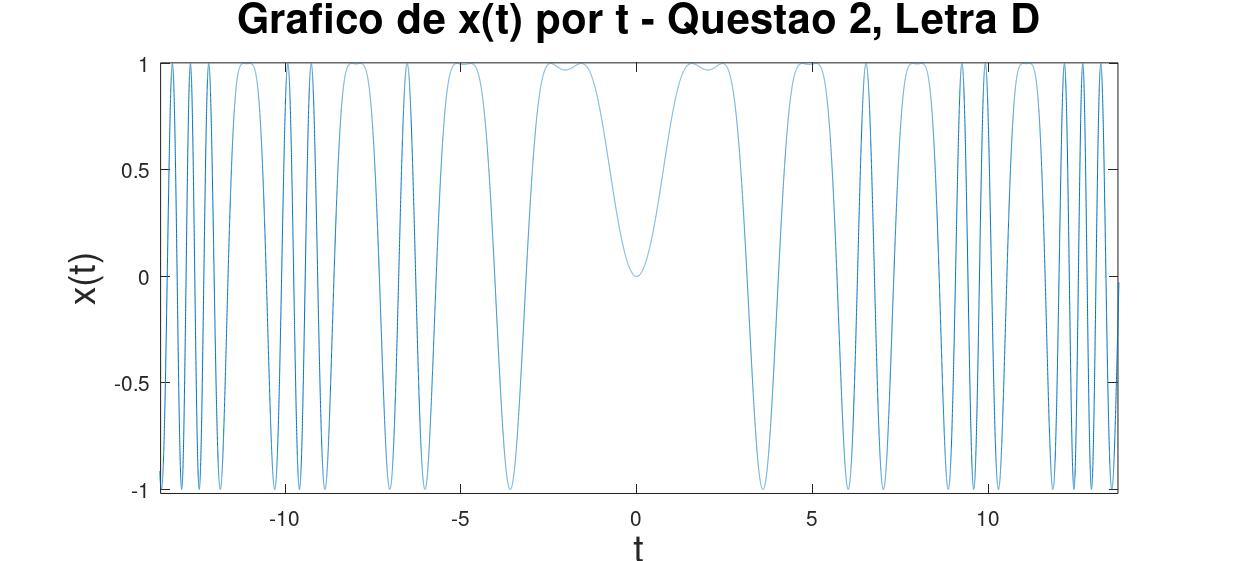
\includegraphics[scale=0.25]{plot2d}
    \centering
\end{figure}

\vspace{\baselineskip}

Do gráfico, nota-se que este sinal não é periódico. As distâncias entre as cristas e entre os vales não é fixa ao longo do gráfico.

\vspace{\baselineskip}

3.) Um sinal periódico com período fundamental $T_{0} = 4 $ é descrito por \textbf{G2}: $x(t) = 1 - e^{|t|}$ para $-T_{0}/2 \leq t < T_{0} / 2$
(a) Esboce o seu gráfico;
(b) calcule analiticamente sua potência total $P$;
(c) calcule $X_{0}$ usando $k = 0$ na fórmula geral de $X_{k}$;
(d) calcule analiticamente os coeficientes $X_{k}$ e verifique se a expressão obtida leva a $X_{0}$ sem indeterminações;
(e) esboce os espectros de módulo e fase;
(f) para $k = 0, 1, 2\;e\;3$, calcule a potência acumulada $P_{k}^{a}$ contida nos harmônicos de $0\;a\;k$;
(g) para $k = 0, 1, 2\;e\;3$, calcule a potência relativa $P_{k}^{a}/P$;
(h) quantos harmônicos são necessários para uma aproximação reter $90.00\%$ da potência?

\vspace{\baselineskip}

(a) Fazendo o esboço do gráfico, teremos:
\begin{figure}[h!]
    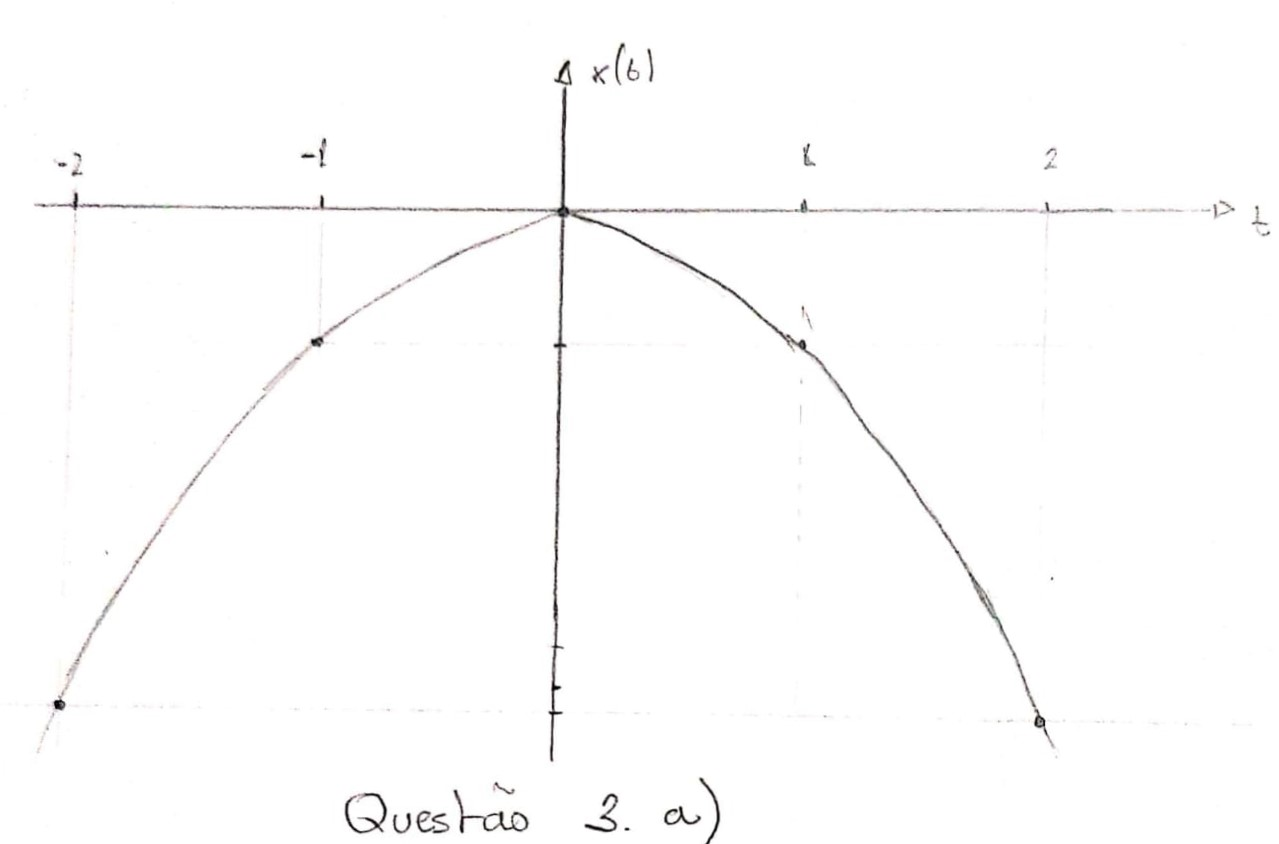
\includegraphics[scale=0.25]{img3a}
    \centering
\end{figure}

\vspace{\baselineskip}

(b) Podemos, inicialmente, calcular a energia do sinal no período $[-2\;2]$ com $T_{0} = 4$ e $\omega_{0} = \frac{2 \pi}{T_{0}} = \frac{\pi}{2}$.\\
$E = \int_{-2}^{2} \mid x(t) \mid ^{2}\,dt = \int_{-2}^{0} \mid 1 - e^{\mid t\mid} \mid^{2}\,dt + \int_{0}^{2} \mid 1 - e^{\mid t\mid} \mid^{2}\,dt$

\[E = \int_{-2}^{0} (1 - 2e^{-t} + e^{-2t})\,dt + \int_{0}^{2} (1 - 2e^{t} + e^{2t})\,dt =\]
\[E = (t + 2e^{-t} - \frac{1}{2}e^{-2t}) \bigg|_{-2}^{0} + (t - 2e^{t} + \frac{1}{2}e^{2t}) \bigg|_{0}^{2} = \]
\[E = (0 +2 - \frac{1}{2} - (-2 + 2e^{2} - \frac{1}{2}e^{4})) + (2 - 2e^{2} + \frac{1}{2}e^{4}) - (0 -2 + \frac{1}{2}) = 7 - 4e^{2} + e^{4}\]
\[E = 7 - 4e^{2} + e^{4}\]
A potência, portanto, será calculada como a energia dividida pelo período de tempo calculado: $P = \frac{7 - 4e^{2} + e^{4}}{4}$.

\vspace{\baselineskip}

(c) A fórmula geral de $X_{k}$ é dada por:
\[X_{k} = \frac{1}{T_{0}} \int_{T_{0}} x(t)\,e^{-jkw_{0}t}\,dt\]
Para o nosso caso:
\[X_{0} = \frac{1}{4} \biggl[\int_{-2}^{0} (1 - e^{-t})\,dt + \int_{0}^{2} (1 - e^{t})\,dt\biggr]\]
\[X_{0} = \frac{1}{4} \biggl[\bigl(t + e^{-t}\bigr)_{-2}^{0} + \bigl(t - e^{t}\bigr)_{0}^{2}\biggr]\]
\[X_{0} = \frac{1}{4} \biggl[\bigl(0 + 1\bigr) - \bigl(-2 + e^{2}\bigr) + \bigl(2 - e^{2}\bigr) - \bigl(0 - 1\bigr)\biggr]\]
\[X_{0} = \frac{3 - e^{2}}{2}\]
O termo DC, vale $\frac{3 - e^{2}}{2}$.

\vspace{\baselineskip}

(d) Já temos a fórmula geral de $X_{k}$ acima descrita. Assim, para o caso geral, temos:
\[X_{k} = \frac{1}{4}\biggl[\int_{-2}^{2} (1 - e^{\mid t \mid})\,e^{-jk\frac{\pi}{2}t}\,dt\biggr]\]

\[X_{k} = \frac{1}{4}\biggl[\int_{-2}^{2} (e^{-jk\frac{\pi}{2}t} - e^{\mid t \mid - jk\frac{\pi}{2}t})\,dt\biggr]\]

\[X_{k} = \frac{1}{4}\biggl[\int_{-2}^{2} e^{-jk\frac{\pi}{2}t}\,dt - \int_{-2}^{2} e^{\mid t \mid - jk\frac{\pi}{2}t}\,dt\biggr]\]

\[X_{k} = \frac{1}{4}\biggl[\int_{-2}^{2} cos(-k\frac{\pi}{2}t) + j\,sen(-k\frac{\pi}{2}t)\,dt - \int_{-2}^{2} e^{\mid t \mid - jk\frac{\pi}{2}t}\,dt\biggr]\]

\[X_{k} = \frac{1}{4}\biggl[\int_{-2}^{2} cos(-k\frac{\pi}{2}t) + j\,sen(-k\frac{\pi}{2}t)\,dt - \int_{-2}^{2} e^{\mid t \mid}(cos(-k\frac{\pi}{2}t) + j\,sen(-k\frac{\pi}{2}t))\,dt\biggr]\]

\[X_{k} = \frac{1}{4}\biggl[\frac{4sen(k\pi)}{k\pi} - \biggl(\int_{-2}^{0} e^{-t}(cos(-k\frac{\pi}{2}t) + j\,sen(-k\frac{\pi}{2}t))\,dt + \int_{0}^{2} e^{t}(cos(-k\frac{\pi}{2}t) + j\,sen(-k\frac{\pi}{2}t))\,dt \biggr)\biggr]\]

\[X_{k} = \frac{1}{4}\biggl[\frac{4sen(k\pi)}{k\pi} - 
\biggl(
    -\frac{2e^{-t}cis(-k\frac{\pi}{2}t)}{2 + jk\pi}\bigg|_{-2}^{0} - 
    \frac{2e^{t}cis(-k\frac{\pi}{2}t)}{jk\pi - 2}\bigg|_{0}^{2}
\biggr)\biggr]\] \textbf{OBS:} $cis(\theta) = cos(\theta) + j\,sen(\theta)$

\[X_{k} = \frac{1}{4}\biggl[\frac{4sen(k\pi)}{k\pi} - 
\biggl(
    \frac{2e^{2}cos(k\pi) - 2}{2 + jk\pi} - 
    \frac{2e^{2}cos(k\pi) - 2}{jk\pi - 2}
\biggr)\biggr]\]

\[X_{k} = \frac{1}{4}\biggl[\frac{4sen(k\pi)}{k\pi} - 
\biggl(
    \frac{8(e^{2}cos(k\pi) - 1)}{4 + k^2\pi^2}
\biggr)\biggr]\]

\[X_{k} = \frac{2 - 2e^2cos(k\pi)}{4 + k^2\pi^2} + \frac{sen(k\pi)}{k\pi}\]

\[X_{k} = \frac{2 - 2e^2cos(k\pi)}{4 + k^2\pi^2} + sinc(k)\]

Agora, é fácil ver que não existem indeterminações para o caso em que $k = 0$.

\vspace{\baselineskip}

(e) Calculado o termo para cada valor de $k$, percebemos que todos são reais. Os reescrevendo:

\[X_{k} = \frac{2 - 2e^2(-1)^{k}}{4 + k^2\pi^2} + sinc(k)\]

vemos que $X_{k}$ assume valores negativos para k par e positivos para k ímpar, fazendo o espectro de fases variar entre os valores $0$ e $\pi$. Dessa forma, fica mais simples expressar o espectro de fases:

Com o auxílio do software Octave, foi possível calcular de maneira mais fácil as magnitudes para os k's pedidos.

\newpage

\begin{figure}[!ht]
    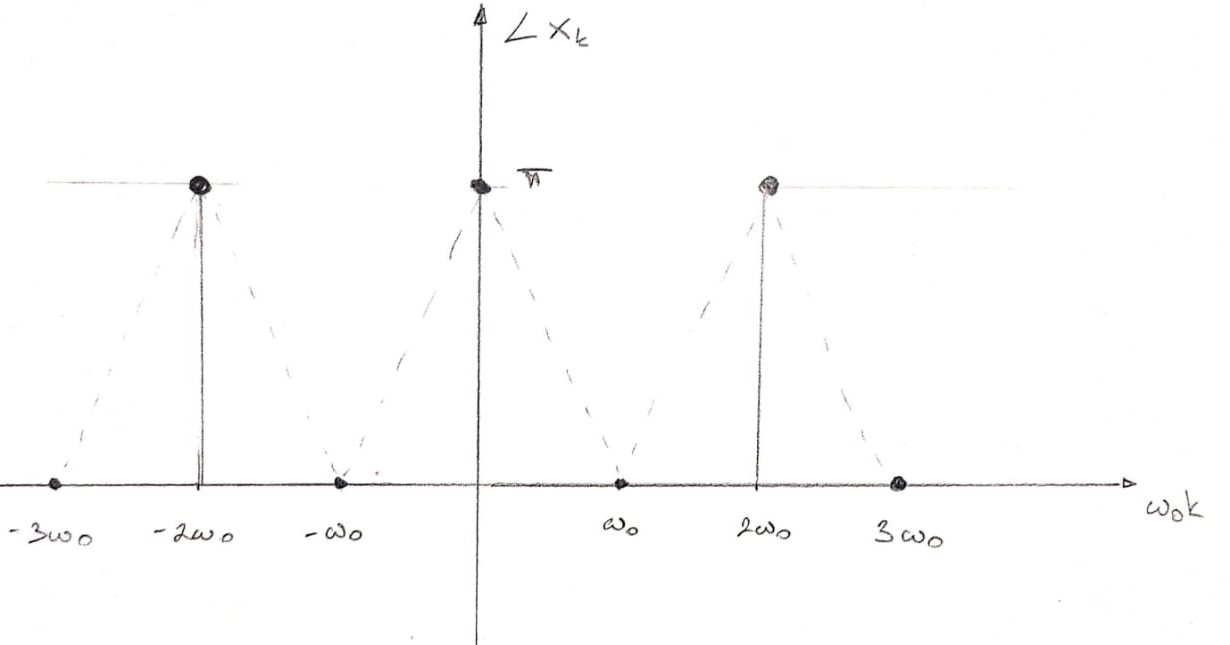
\includegraphics[scale=0.25]{img3e_fase}
    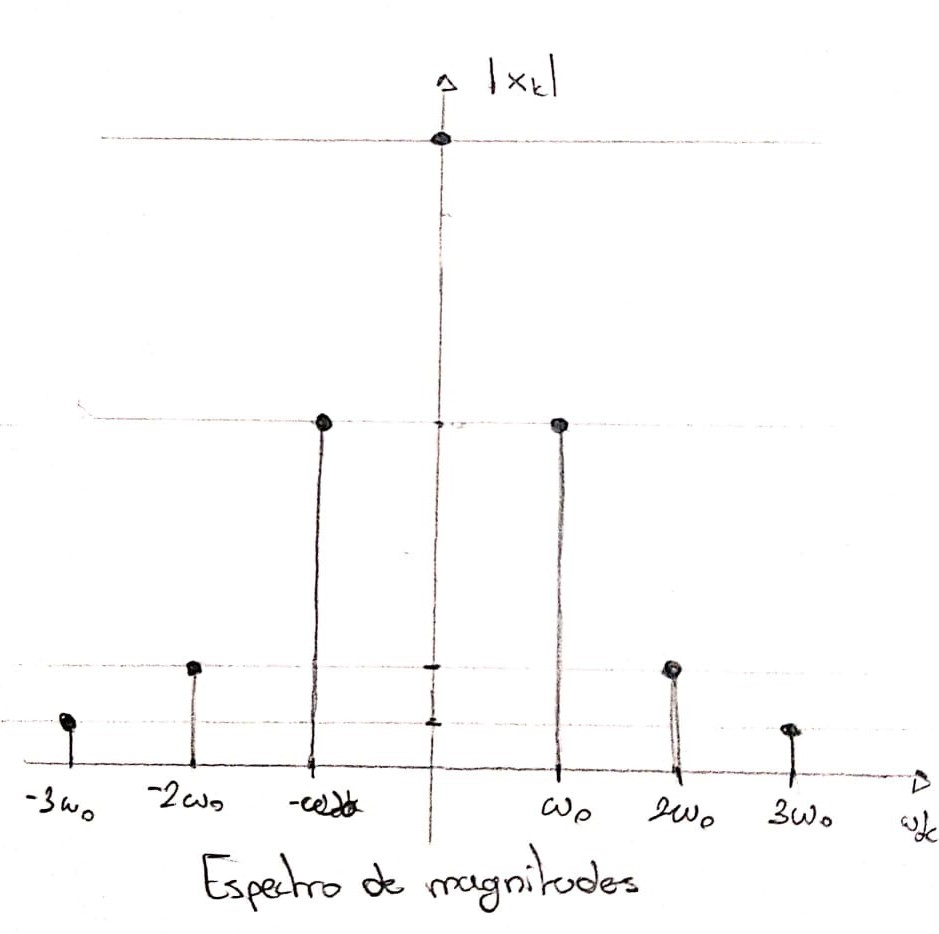
\includegraphics[scale=0.25]{img3e_mag}
    \centering
\end{figure}

\vspace{\baselineskip}

(f) Com o auxílio do Octave, calculamos as potências acululadas nos harmônicos de 0 até 3:
\[P_{1--3} = 7.9808\]

\vspace{\baselineskip}

(g) Também com o auxílio do Octave, calculamos as potências relativas (Lembrando que a potência total foi dada por: $\frac{7 - 4e^{2} + e^4}{4} = 8.0105$):

A potência para o harmônico k, é facilmente calculada como $2\mid X_{k} \mid^{2}$ para $k \neq 0$.
\begin{align*}
    P_{0} &= 60.12\%\\
    P_{1} &= 36.53\%\\
    P_{2} &= 2.15\%\\
    P_{3} &= 0.81\%
\end{align*}

(h) Do item acima, nota-se que já no segundo harmônico, a potência atinge $96.65\%$. Sendo assim, são necessários apenas dois harmônicos.

\vspace{\baselineskip}

4.) O grupo $i$ trabalhará com o sinal periódico $x(t)$ usado pelo grupo $i + 1$ na questão 1 (ao grupo 7: sinal 1). As aproximações numéricas para Octave/MatLab vistas, podem e devem ser utilizadas.
(a) Traçar gráfico;
(b) encontrar potência total $P$;
(c) calcular os $X_{k}$ para $k \in [-10\;10]$;
(d) traçar os espectos de magnitude, fase e potência;
(e) estimar quantos harmônicos são necessários para reter $90.00\%$ da potência;
(f) calcular os coeficientes $a_{k}\;e\;b_{k}$ correspondentes;
(g) traçar, num mesmo gráfico, $x(t)$ e as aproximações.

Sinal a ser estudado: {\textbf G3}: $x(t) = -t - 5, -2, -t^3 + 3t, 2, -t + 5$ para o intervalo $I_{1} = [-5\;-3], I_{2} = [-3\;-1], I_{3} = [-1\;1], I_{4} = [1\;3], I_{5} = [3\;5]$.

(a) Traçando o gráfico do sinal periódico:

\begin{figure}[!ht]
    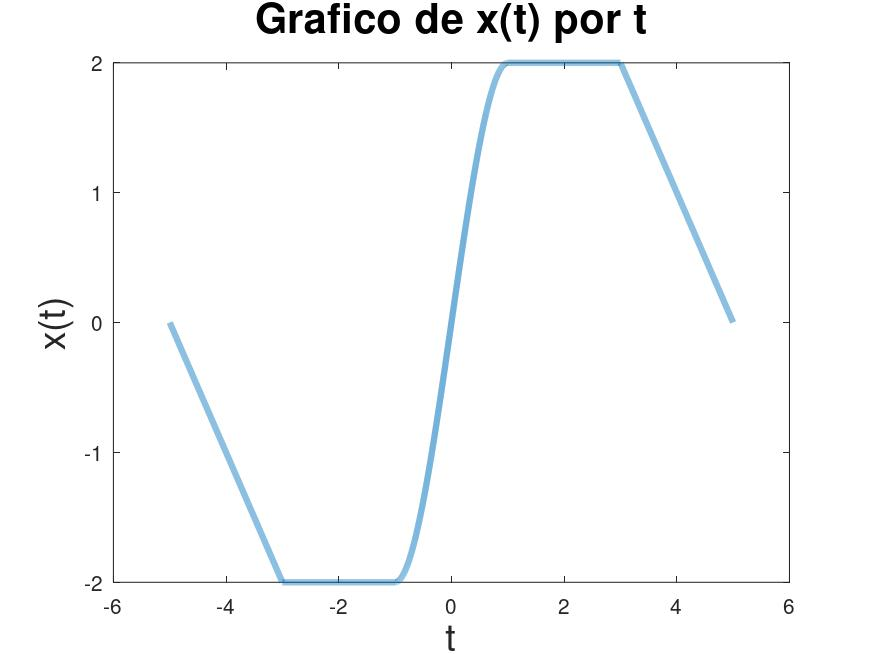
\includegraphics[scale=0.2]{plot4a}
    \centering
\end{figure}

\vspace{\baselineskip}

(b) Encontrando a potência total $P$ com a aproximação da fórmula $P_{[-5\;5]} = \frac{1}{5 - (-5)} \int_{-5}^{5} |x(t)|^2 dt $:

\vspace{\baselineskip}

Potência total $(P)$ = 2.5219

\vspace{\baselineskip}

(c) Calculando os $X_{k}$ para $k \in [-10\;10]$:

\begin{align*}
    X_{-10} &=  3.6250 \times 10^{-17} - 4.8377\times 10^{-3}j; & X_{10} &=  3.6250\times 10^{-17} + 4.8377\times 10^{-3}j.\\
    X_{-9} &=  1.3859\times 10^{-18} - 1.2007\times 10^{-2}j;   & X_{9} &=  1.3859\times 10^{-18} + 1.2007\times 10^{-2}j;\\
    X_{-8} &=  1.5344\times 10^{-17} - 5.4810\times 10^{-5}j;   & X_{8} &=  1.5344\times 10^{-17} + 5.4810\times 10^{-5}j;\\
    X_{-7} &= -1.1824\times 10^{-18} + 7.3857\times 10^{-3}j;   & X_{7} &= -1.1824\times 10^{-18} - 7.3857\times 10^{-3}j;\\
    X_{-6} &= -3.0899\times 10^{-17} + 1.2438\times 10^{-3}j;   & X_{6} &= -3.0899\times 10^{-17} - 1.2438\times 10^{-3}j;\\
    X_{-5} &=  1.6911\times 10^{-17} + 3.8702\times 10^{-2}j;   & X_{5} &=  1.6911\times 10^{-17} - 3.8702\times 10^{-2}j;\\
    X_{-4} &=  3.1526\times 10^{-17} + 1.0894\times 10^{-1}j;   & X_{4} &=  3.1526\times 10^{-17} - 1.0894\times 10^{-1}j;\\
    X_{-3} &= -6.7537\times 10^{-18} + 1.1269\times 10^{-1}j;   & X_{3} &= -6.7537\times 10^{-18} - 1.1269\times 10^{-1}j;\\
    X_{-2} &=  1.4539\times 10^{-17} + 1.9635\times 10^{-1}j;   & X_{2} &=  1.4539\times 10^{-17} - 1.9635\times 10^{-1}j;\\
    X_{-1} &=  1.4886\times 10^{-17} + 1.0936j;                  & X_{1} &=  1.4886\times 10^{-17} - 1.0936j;\\
    X_{o} &= 6.3307\times 10^{-17}; &
\end{align*}

(d) Traçando os espectros de magnitude, fase e potência:

\begin{figure}[h!]
    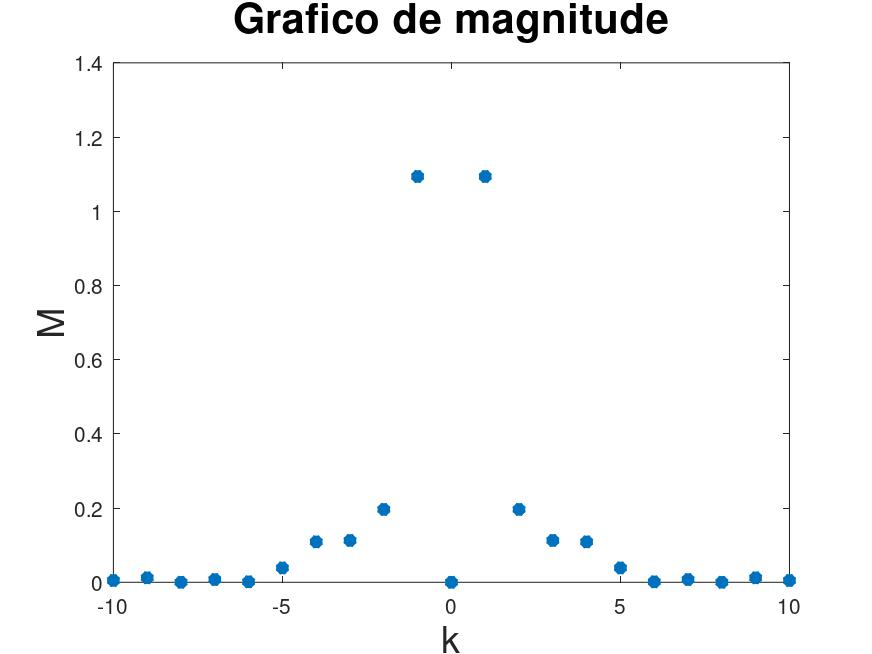
\includegraphics[scale=0.25]{plot4dm}
    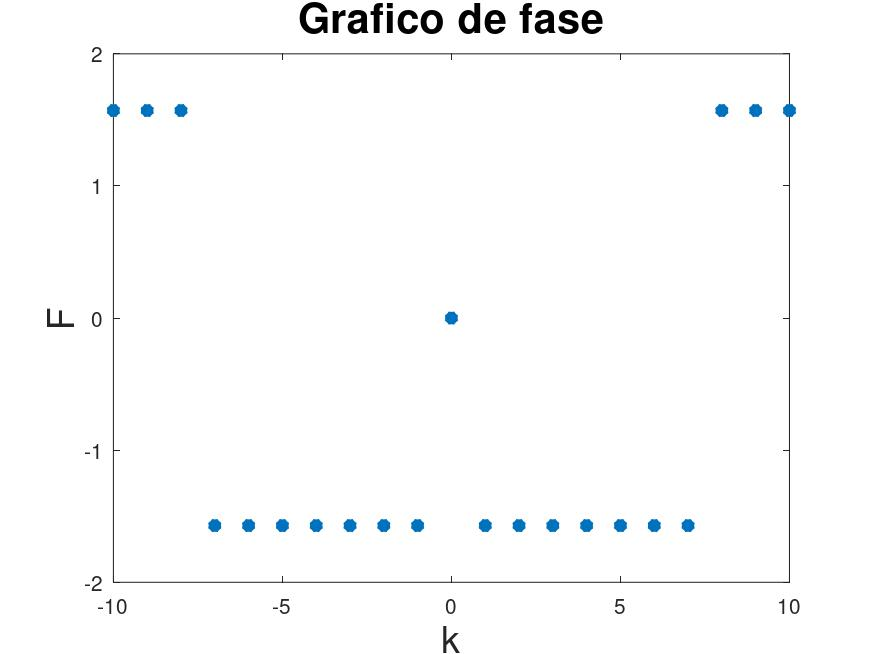
\includegraphics[scale=0.25]{plot4df}
    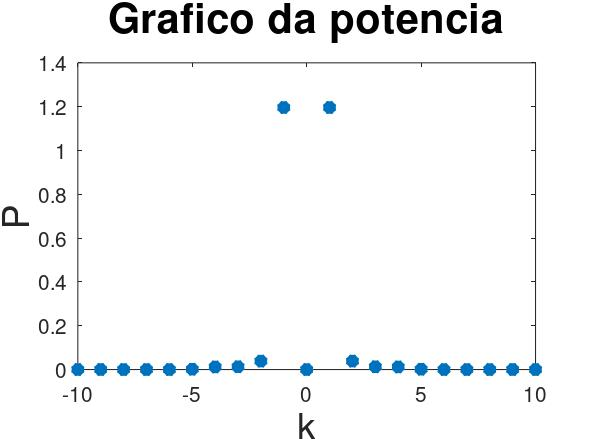
\includegraphics[scale=0.4]{plot4dp}
\end{figure}

\vspace{\baselineskip}

(e) Estimando quantos harmônicos são necessários para reter $90.00\%$ da potência:

\vspace{\baselineskip}

Dois harmônicos para alcançar $94,85\% $ da potência.

\vspace{\baselineskip}

(f) Calculando $a_{k}$ e $b_{k}$ a partir dos coeficientes $X_{k}$, teremos:

\begin{align*}
    a_{k} = X_{k} + X_{-k}\\
    b_{k} = j(X_{k} - X_{-k})
\end{align*}

\begin{align*}
    a_{0} &= 6.3307\times 10^{-17}   &   b_{0} &= 0\\
    a_{1} &= 2.9772\times 10^{-17}   &   b_{1} &= 2.1873\\
    a_{2} &= 2.9078\times 10^{-17}   &   b_{2} &= 0.3927\\
    a_{3} &= -1.3507\times 10^{-17}  &   b_{3} &= 0.2254\\
    a_{4} &= 6.3052\times 10^{-17}   &   b_{4} &= 0.2179\\
    a_{5} &= 3.3822\times 10^{-17}   &   b_{5} &= 0.077404\\
    a_{6} &= -6.1798\times 10^{-17}  &   b_{6} &= 2.4876\times 10^{-3}\\
    a_{7} &= -2.3649\times 10^{-18}  &   b_{7} &= 0.014771\\
    a_{8} &= 3.0689\times 10^{-17}   &   b_{8} &= -1.0962\times 10^{-4}\\
    a_{9} &= 2.7717\times 10^{-18}   &   b_{9} &= -0.024014\\
    a_{10} &= 7.2500\times 10^{-17}  &   b_{10} &= -9.6755\times 10^{-3}
\end{align*}

5.) Na escala de tempo {\tt t=0:1/2000:5}, considere um sinal de áudio simples $x_{b}(t) = sen(2 \pi f_{0}t)$ ou $x_{b}(t) = cos(2 \pi f_{0}t)$ com frequência \textbf{G2:} $f_{0} = 132Hz$. Ouça este som usando o comando {\tt sound(xb)} no Octave; o resultado é, provavelmente, desagradável pois se trata de uma frequência pura e a sensação é seca, metálica. Para melhorar o \textbf{timbre} do som é preciso colocar mais harmônicos. Crie, na mesma escala de tempo, com a mesma frequência fundamental $f_{0}$, com parâmetros a seu critério e usando até o harmônico $k = 6\;(6f_{0}Hz)$ os sinais a seguir. Ouça cada um deles e compare a qualidade do timbre.\\
(a) Uma onda quadrada $x_{q}(t)$;
(b) uma onda triangular $x_{t}(t)$;
(c) um seno semi-retificado sem o nível DC $x_{s}(t)$;
(d) Opcional: adicionando senos e co-senos harmônicos a seu critério, imagine-se projetando um sintetizador de som e crie um sinal periódico $x(t)$ com frequência fundamental $f_{0}$ e um timbre agradável.

\textbf{Como aqui as respostas são os próprios códigos, preferimos adicioná-los logo abaixo do enunciado.}\\
{\centering \textbf{Letra A}}

\begin{verbatim}
%% Programa da quinta questao do trabalho de Sinais e Sistemas
%% 2022.2

% dados basicos
f0=132; soma=0;
dt=1/2000;
t=0:dt:5;
var=2*pi*f0*t;

% Gerando o sinal
soma = 0;
for i=0:1:5;
    a=2*i+1;
    xq=sin(a*var)/a;
    soma=soma+xq;
end
sound(soma);
\end{verbatim}

\vspace{\baselineskip}

{\centering \textbf{Letra B}}
\begin{verbatim}
%% Programa da quinta questao do trabalho de Sinais e Sistemas
%% 2022.2

% dados basicos
dt=0.001;
soma=0;
f0=132; var=(2*pi*f0);
A=1; cte=8*A/(pi*pi);
t=-2:dt:2;

% Gerando o sinal
for i=0:5,
    a=2*i+1;
    xt=(cte/(a*a)).*cos(a*var*t);
    soma=soma+xt;
end;

sound(soma);
\end{verbatim}

\vspace{\baselineskip}

{\centering \textbf{Letra C}}
\begin{verbatim}
%% Programa da quinta questao do trabalho de Sinais e Sistemas
%% 2022.2

% dados basicos
A=1;f0=132;w0=2*pi*f0;cossenos=0;
dt=1/2000; t=0:dt:5;

% gerando o sinal
for i=1:6,
    n=2*i;
    soma=(2*A/(pi*(power(n,2)-1))).*cos(n*w0*t);
    cossenos = soma + cossenos;
end;
xs = (A/2)*sin(w0*t) - cossenos;
sound(xs);
\end{verbatim}

\newpage

Ao longo do trabalho, nós utilizamos o software Octave para plotar gráficos e calcular dados de maneira mais precisa. Assim, como muitos deles faziam parte do próprio trabalho, decidimos anexá-los ao final.

\vspace{\baselineskip}

{\textbf{Códigos para a questão 1}}
\begin{verbatim}
% Programa da primeira questao do trabalho de sinais e sistemas
% 2022.2

% Intervalos
dt=0.001;

% Dados basicos
t1=-5:dt:-3-dt; x1=0*t1-3;
t2=-3:dt:-1-dt; x2=3*t2+6;
t3=-1:dt:1-dt; x3=-3*t3.^3;
t4=1:dt:3-dt; x4=3*t4-6;
t5=3:dt:5-dt; x5=-t5.^2+5*t5-3;

% Concatenando e plotando
t=[t1 t2 t3 t4 t5]; x=[x1 x2 x3 x4 x5];
plot(t, x, "r", "linewidth", 3);

title("Grafico de x(t) por t - Questao 1", "fontsize", 20);
xlabel("t", "fontsize", 18);
ylabel("x(t)", "fontsize", 18);
\end{verbatim}

\vspace{\baselineskip}

{\textbf{Códigos para a questão 2}}
\textbf{a)}
\begin{verbatim}
% Programa da segunda questao do trabalho de sinais e sistemas
% 2022.2

% Intervalo
dt=0.001;

%   Letra a)
% Dados basicos
t=-5:dt:5-dt; x=sin(pi*t)+cos(2*pi*t)/2+sin(3*pi*t)/3+cos(4*pi*t)/4;
plot (t, x);
title("Grafico de x(t) por t - Questao 2, Letra A", "fontsize", 20);
xlabel("t", "fontsize", 18);
ylabel("x(t)", "fontsize", 18);
\end{verbatim}

\noindent \textbf{b)}
\begin{verbatim}
% Programa da segunda questao do trabalho de sinais e sistemas
% 2022.2

% Intervalo
dt=0.001;

%   Letra b)
% Dados basicos
w=1;
t=-7:dt:7-dt; x=sin(w*t).*cos(50*w*t);

% Plotando
plot (t, x);
title("Grafico de x(t) por t - Questao 2, Letra B", "fontsize", 20);
xlabel("t", "fontsize", 18);
ylabel("x(t)", "fontsize", 18);
\end{verbatim}

\noindent \textbf{c)}
\begin{verbatim}
% Programa da segunda questao do trabalho de sinais e sistemas
% 2022.2

% Intervalo
dt=0.001;

%   Letra c)
w=1;
t=-15:dt:15-dt; x=sin(w*(t.^2));

% Plotando
plot(t,x);
title("Grafico de x(t) por t - Questao 2, Letra C", "fontsize", 20);
xlabel("t", "fontsize", 18);
ylabel("x(t)", "fontsize", 18);
\end{verbatim}

\noindent \textbf{d)}
\begin{verbatim}
% Programa da segunda questao do trabalho de sinais e sistemas
% 2022.2

% Intervalo
dt=0.001;

%   Letra d)
w1=1;
w2=1;
t=-15:dt:15-dt; x=sin(w1.*sin(w2*t).*t);

% Plotando
plot(t,x);
title("Grafico de x(t) por t - Questao 2, Letra D", "fontsize", 20);
xlabel("t", "fontsize", 18);
ylabel("x(t)", "fontsize", 18);
\end{verbatim}

\vspace{\baselineskip}

{\textbf{Códigos para a questão 3}}
\begin{verbatim}
%% Encontrando o Xk correto

dt = 0.001;
t = -2:dt:2-dt;
x = (1 - exp(abs(t)));

Xk = zeros(1, 7);
for k = -3:1:3;
    Xk(k + 4) = ((2 - 2*exp(2)*cos(k * pi))/(4 + (k*pi)^2)) + sinc(k);
end

disp(Xk);

% Magnitude
M = zeros(1, 7);
for k = 1:1:7;
    M(k) = abs(Xk(k));
end

disp(M);

% Potencia
P = zeros(1, 4);
for k = 1:1:4;
    P(k) = M(k + 3)^2;
end
for k = 2:1:4;
    P(k) = P(k) * 2;
end

disp(P);

disp("Potencia acumulada:"), disp(sum(P));

% Potencia total
P_total = (7 - 4*exp(2) + exp(4))/4;

% Potencias relativas
P_rel = P/P_total
\end{verbatim}

\vspace{\baselineskip}

{\textbf{Códigos para a questão 4}}
\begin{verbatim}
% Programa da quarta questao do trabalho de sinais e sistemas
% 2022.2

% Intervalos
dt=0.001;
T0 = 10;
w0 = 2*pi/T0;

% Dados basicos
t1=-5:dt:-3-dt; x1=-t1-5;
t2=-3:dt:-1-dt; x2=0*t2-2;
t3=-1:dt:1-dt; x3=-t3.^3+3*t3;
t4=1:dt:3-dt; x4=0*t4+2;
t5=3:dt:5-dt; x5=-t5+5;

% Concatenando e plotando
t=[t1 t2 t3 t4 t5]; x=[x1 x2 x3 x4 x5];
%plot(t, x, "-", "linewidth", 3)
%title("Grafico de x(t) por t", "fontsize", 20)
%xlabel("t", "fontsize", 18)
%ylabel("x(t)", "fontsize", 18)
%print plot4a.jpg

% Encontrando a potencia total P
Ptotal = sum(abs(x).^2*dt)/T0;

% Encontrando os Xk para k pertence a [-10 10]
xk0 = sum(x.*exp(-i*0*w0.*t)*dt)/T0;
xk1 = sum(x.*exp(-i*1*w0.*t)*dt)/T0;
xk2 = sum(x.*exp(-i*2*w0.*t)*dt)/T0;
xk3 = sum(x.*exp(-i*3*w0.*t)*dt)/T0;
xk4 = sum(x.*exp(-i*4*w0.*t)*dt)/T0;
xk5 = sum(x.*exp(-i*5*w0.*t)*dt)/T0;
xk6 = sum(x.*exp(-i*6*w0.*t)*dt)/T0;
xk7 = sum(x.*exp(-i*7*w0.*t)*dt)/T0;
xk8 = sum(x.*exp(-i*8*w0.*t)*dt)/T0;
xk9 = sum(x.*exp(-i*9*w0.*t)*dt)/T0;
xk10 = sum(x.*exp(-i*10*w0.*t)*dt)/T0;

k = [-10:10];
magnitude = [abs(xk10) abs(xk9) abs(xk8) abs(xk7) abs(xk6) abs(xk5) abs(xk4) abs(xk3)\
            abs(xk2) abs(xk1) abs(xk0) abs(xk1) abs(xk2) abs(xk3) abs(xk4) abs(xk5)\
            abs(xk6) abs(xk7) abs(xk8) abs(xk9) abs(xk10)];
fase = [arg(xk10) arg(xk9) arg(xk8) arg(xk7) arg(xk6) arg(xk5) arg(xk4) arg(xk3) arg(xk2)\
        arg(xk1) arg(xk0) arg(xk1) arg(xk2) arg(xk3) arg(xk4) arg(xk5) arg(xk6) arg(xk7)\
        arg(xk8) arg(xk9) arg(xk10)];
%subplot(2,2,2)
%plot(k, magnitude, "*", "linewidth", 3)
%title("Grafico de magnitude", "fontsize", 20)
%xlabel("k", "fontsize", 18)
%ylabel("M", "fontsize", 18)
%print plot4dm.jpg

%subplot(2,2,3)
%plot(k, fase, "*", "linewidth", 3)
%title("Grafico de fase", "fontsize", 20)
%xlabel("k", "fontsize", 18)
%ylabel("F", "fontsize", 18)
%print plot4df.jpg

% Encontrando a potencia de cada Xk
P0 = abs(xk0)^2;
P1 = abs(xk1)^2;
P2 = abs(xk2)^2;
P3 = abs(xk3)^2;
P4 = abs(xk4)^2;
P5 = abs(xk5)^2;
P6 = abs(xk6)^2;
P7 = abs(xk7)^2;
P8 = abs(xk8)^2;
P9 = abs(xk9)^2;
P10 = abs(xk10)^2;

P = [P10 P9 P8 P7 P6 P5 P4 P3 P2 P1 P0 P1 P2 P3 P4 P5 P6 P7 P8 P9 P10];
%subplot(2,2,4)
%plot(k, P, "*", "linewidth", 3)
%title("Grafico da potencia", "fontsize", 20)
%xlabel("k", "fontsize", 18)
%ylabel("P", "fontsize", 18)
%print plot4dp.jpg

% Estimando a quantidade de harmonicos necessarios para reter 90% da potencia total
p = abs(sum(x.*exp(-i*0*w0.*t)*dt)/T0)^2/Ptotal;
harmonico = 1;
while (p < 0.9)
    p = p + 2*abs(sum(x.*exp(-i*harmonico*w0.*t)*dt)/T0)^2/Ptotal
    harmonico++
endwhile

a0 = xk0;
a1 = (xk1+conj(xk1));
a2 = (xk2+conj(xk2));
a3 = (xk3+conj(xk3));
a4 = (xk4+conj(xk4));
a5 = (xk5+conj(xk5));
a6 = (xk6+conj(xk6));
a7 = (xk7+conj(xk7));
a8 = (xk8+conj(xk8));
a9 = (xk9+conj(xk9));
a10 = (xk10+conj(xk10));

b0 = i*(xk0-conj(xk0));
b1 = i*(xk1-conj(xk1));
b2 = i*(xk2-conj(xk2));
b3 = i*(xk3-conj(xk3));
b4 = i*(xk4-conj(xk4));
b5 = i*(xk5-conj(xk5));
b6 = i*(xk6-conj(xk6));
b7 = i*(xk7-conj(xk7));
b8 = i*(xk8-conj(xk8));
b9 = i*(xk9-conj(xk9));
b10 = i*(xk10-conj(xk10));

% Tracando grafico de x(t) e aproximacoes
plot(t, x), hold on
f0 = xk0.*exp(i*0*w0.*t);
plot(t, f0), hold on
f1 = xk0.*exp(i*0*w0.*t) + xk1.*exp(i*1*w0.*t) + conj(xk1).*exp(i*1*w0.*t);
plot(t, f1)
\end{verbatim}


\end{document}
